\chapter{Métrica, expansión y una primera cosmología}

Al final de la clase anterior habíamos llegado a una ecuación de ondas invariante de Lorentz y nos disponíamos a escribir las ecuaciones de Maxwell en forma espaciotemporal. Una pregunta del público nos da ahora una advertencia útil antes de pasar a la gravitación: ¿hasta qué punto puede la simetría determinar por sí sola una teoría física? La respuesta es tajante: mucho, pero no todo. La invariancia de Lorentz es un poderoso filtro para las leyes posibles. No sustituye los demás supuestos físicos ni los experimentos.

\section{Lo que la simetría no determina}

\begin{classroomqa}
\audiencequestion{Una vez que sabemos que los campos eléctrico y magnético se transforman conjuntamente bajo las transformaciones de Lorentz, ¿se deducen las ecuaciones de Maxwell solo de la relatividad?}
\lecturerresponse{No. La relatividad restringe la forma de las ecuaciones, pero para construirlas también se recurre a su linealidad, al bajo orden de sus derivadas, a la manera en que se transforman los campos y a la información experimental. Sin esos ingredientes adicionales, seguirían siendo posibles muchas ecuaciones de campo covariantes de Lorentz.}
\end{classroomqa}

El supuesto adicional más importante para esta introducción es la linealidad. Si \(A(x,t)\) es una solución de una ecuación de campo lineal, entonces \(\lambda A(x,t)\) también lo es para cualquier constante \(\lambda\). Si \(A\) y \(B\) son soluciones, entonces también lo es \begin{equation}
  C(x,t)=A(x,t)+B(x,t).
  \label{eq:superposition}
\end{equation}
Este es el principio de superposición. Dos ondas electromagnéticas sin fuentes pueden cruzarse y salir intactas. No chocan directamente como lo hacen los objetos materiales. Pueden interactuar indirectamente a través de la materia cargada, porque cada onda mueve las cargas y las cargas en movimiento emiten radiación; sin embargo, las propias ecuaciones de campo en el vacío son lineales.

\begin{figure}[H]
\centering
\includegraphics[width=0.64\textwidth]{lecture_08_figure_01.png}
\caption{Dos perfiles de onda en la pizarra durante la explicación de la superposición. Su suma vuelve a ser una onda sin fuentes admisible.}
\lectureframe{00:05:30}
\end{figure}

El oscilador armónico hace transparente el álgebra. Supongamos que \begin{equation}
  m\ddot x=-kx.
  \label{eq:linear-oscillator}
\end{equation}
Si \(x_1\) y \(x_2\) satisfacen \eqref{eq:linear-oscillator}, entonces \begin{equation}
  m(\ddot x_1+\ddot x_2)
  =-k(x_1+x_2),
\end{equation}
por lo que \(x_1+x_2\) es una solución. Sin embargo, si añadimos un término no lineal, \begin{equation}
  m\ddot x=-kx+p x^2,
  \label{eq:nonlinear-oscillator}
\end{equation}
la suma ya no funciona:
\begin{equation}
  (x_1+x_2)^2=x_1^2+x_2^2+2x_1x_2.
\end{equation}
El término cruzado \(2x_1x_2\) no tiene un término correspondiente en las dos ecuaciones por separado. Ahora los dos movimientos se influyen mutuamente.

\begin{figure}[H]
\centering
\includegraphics[width=0.73\textwidth]{lecture_08_figure_02.png}
\caption{Comparación entre las ecuaciones de los osciladores por separado y la ecuación para su suma. El término cuadrático deja al descubierto el término cruzado adicional que rompe la superposición.}
\lectureframe{00:10:10}
\end{figure}

Este ejemplo fija el punto metodológico que se mantendrá durante toda la exposición sobre cosmología. La simetría nos dice qué magnitudes pueden combinarse y qué ecuaciones son admisibles. La dinámica y la observación nos dicen cuál de las ecuaciones admisibles utiliza la naturaleza.

\section{El intervalo como geometría}

Dejamos ahora el electromagnetismo y tomamos un breve camino hacia la relatividad general y la cosmología. El objeto de partida es el intervalo entre sucesos vecinos. Etiquetemos un suceso con cuatro coordenadas \(x^\mu\) y un suceso cercano con \(x^\mu+dx^\mu\). En coordenadas cartesianas inerciales, con \(c=1\) y la convención \((+,-,-,-)\),
\begin{equation}
  d\tau^2
  =dt^2-dx^2-dy^2-dz^2
  =dx^\mu dx_\mu
  =\eta_{\mu\nu}\,dx^\mu dx^\nu.
  \label{eq:minkowski-interval}
\end{equation}
La cantidad invariante es \(d\tau^2\), no una diferencia de coordenadas particular. Las transformaciones de Lorentz cambian \(dt,dx,dy,dz\), pero conservan esta combinación cuadrática. Por tanto, la relatividad especial puede entenderse como la geometría del espaciotiempo de Minkowski.

\begin{figure}[H]
\centering
\includegraphics[width=0.72\textwidth]{lecture_08_figure_03.png}
\caption{El intervalo de Minkowski escrito sucesivamente en notación por componentes, con índices contraídos y con el tensor métrico.}
\lectureframe{00:14:50}
\end{figure}

La sencillez de \eqref{eq:minkowski-interval} depende de las coordenadas. Incluso un plano llano puede adquirir coeficientes poco familiares si lo etiquetamos de manera poco conveniente. Supongamos que \(x\) se mide en centímetros y \(y\) en metros. Para un desplazamiento físico,
\begin{equation}
  ds^2=dx^2+\left(\frac{dy}{100}\right)^2
      =dx^2+10^{-4}dy^2.
  \label{eq:mixed-units}
\end{equation}
El factor \(10^{-4}\) no dice nada sobre la curvatura. Solo convierte entre unidades.

\begin{figure}[H]
\centering
\includegraphics[width=0.59\textwidth]{lecture_08_figure_04.png}
\caption{Un plano llano descrito con centímetros en un eje y metros en el otro. Los coeficientes métricos desiguales codifican las unidades, no la curvatura.}
\lectureframe{00:20:10}
\end{figure}

Las coordenadas oblicuas añaden un término mixto. En dos dimensiones, la forma cuadrática local más general puede escribirse como
\begin{align}
  ds^2
  &=a_{11}\,dx^2+a_{12}\,dx\,dy\notag\\
  &\quad+a_{21}\,dy\,dx+a_{22}\,dy^2,
  \qquad a_{12}=a_{21}.
  \label{eq:quadratic-form}
\end{align}
Como los diferenciales ordinarios conmutan, \(dx\,dy=dy\,dx\), solo contribuye la parte simétrica de la matriz de coeficientes. Reunimos los coeficientes en la matriz
\begin{equation}
  g=
  \begin{pmatrix}
    a_{11} & a_{12}\\
    a_{21} & a_{22}
  \end{pmatrix}.
  \label{eq:metric-matrix}
\end{equation}
Esta matriz es la \emph{métrica}. Es la regla local que convierte las diferencias de coordenadas en intervalos físicos.

\begin{figure}[H]
\centering
\includegraphics[width=0.71\textwidth]{lecture_08_figure_05.png}
\caption{La forma diferencial cuadrática y su matriz simétrica de coeficientes \(2\times2\) en el momento en que se identifica la matriz como la métrica.}
\lectureframe{00:24:07}
\end{figure}

Las cuadrículas rectangulares o oblicuas uniformes tienen coeficientes constantes. Si las líneas de coordenadas se curvan, se apiñan o se separan, esos coeficientes pasan a ser funciones de la posición, aunque la superficie subyacente siga siendo plana. La notación general para el espaciotiempo es
\begin{equation}
  ds^2=g_{\mu\nu}(x)\,dx^\mu dx^\nu.
  \label{eq:general-metric}
\end{equation}

\begin{figure}[H]
\centering
\includegraphics[width=0.66\textwidth]{lecture_08_figure_06.png}
\caption{La métrica general dependiente de la posición, una vez que se permite que la cuadrícula de coordenadas varíe de un punto a otro.}
\lectureframe{00:28:10}
\end{figure}

Conocer \(g_{\mu\nu}\) en un sistema de coordenadas dado determina las distancias, los tiempos y los ángulos locales y, con ello, determina la geometría. La recíproca no es única: una misma geometría tiene infinitas descripciones en coordenadas y, por tanto, infinitas matrices de funciones coeficientes relacionadas mediante transformaciones de coordenadas.

\section{Complejidad de las coordenadas y curvatura intrínseca}

Ahora debemos distinguir una métrica complicada de un espacio curvo. Enrolla una hoja de papel para formar un cilindro sin estirarla. Su aspecto en la habitación cambia, pero todas las distancias medidas sobre la hoja siguen siendo las mismas. Una criatura confinada al papel no puede detectar el doblamiento mediante ninguna medición intrínseca. Ese es un doblamiento extrínseco, no la curvatura a la que nos referimos aquí.

Una semiesfera es distinta. No se puede aplanar sin estirarla, rasgarla o comprimirla. Todo mapa plano de la Tierra debe deformar la distancia, el área, los ángulos o alguna combinación de estos. Este impedimento es intrínseco y puede detectarse sin observar una dimensión circundante.

Las coordenadas polares ofrecen el contraejemplo plano indispensable. En un plano, un desplazamiento radial infinitesimal tiene longitud \(dr\), mientras que un desplazamiento angular \(d\theta\) a distancia radial \(r\) tiene longitud \(r\,d\theta\). Así,
\begin{equation}
  ds^2=dr^2+r^2d\theta^2,
  \qquad
  g_{\text{polar}}=
  \begin{pmatrix}
    1&0\\
    0&r^2
  \end{pmatrix}.
  \label{eq:polar-metric}
\end{equation}
El coeficiente \(r^2\) varía por todo el plano, pero el plano es llano. El cambio de variables
\begin{equation}
  x=r\cos\theta,\qquad y=r\sin\theta
\end{equation}
recupera la métrica constante \(ds^2=dx^2+dy^2\).

\begin{figure}[H]
\centering
\includegraphics[width=0.70\textwidth]{lecture_08_figure_07.png}
\caption{La métrica polar y su transformación de vuelta a la métrica cartesiana. La matriz dependiente de la posición de la izquierda sigue describiendo un plano llano.}
\lectureframe{00:39:20}
\end{figure}

\begin{classroomqa}
\audiencequestion{¿Debería aparecer un seno en la distancia angular en coordenadas polares?}
\lecturerresponse{No en el plano. Allí, la longitud del arco es \(r\,d\theta\). El seno aparece en la esfera, donde un círculo de latitud tiene radio \(R\sin\theta\).}
\end{classroomqa}

Consideremos una esfera de radio \(R\). Sea \(\theta\) el ángulo polar medido desde el polo norte y \(\phi\) el ángulo acimutal. Un desplazamiento a lo largo de un meridiano tiene longitud \(R\,d\theta\). Para un ángulo polar \(\theta\), el círculo de latitud tiene radio \(R\sin\theta\), por lo que un desplazamiento acimutal tiene longitud \(R\sin\theta\,d\phi\). El teorema de Pitágoras local da
\begin{align}
  ds^2
  &=R^2\left(d\theta^2+\sin^2\theta\,d\phi^2\right),
  \label{eq:sphere-metric}\\
  g_{\text{sphere}}=
  &\begin{pmatrix}
    R^2&0\\
    0&R^2\sin^2\theta
  \end{pmatrix}.
\end{align}

\begin{figure}[H]
\centering
\includegraphics[width=0.72\textwidth]{lecture_08_figure_08.png}
\caption{La esfera, su elemento de línea angular y la matriz métrica correspondiente. El factor \(\sin^2\theta\) representa la disminución del tamaño de los círculos de latitud.}
\lectureframe{00:45:15}
\end{figure}

\begin{figure}[H]
\centering
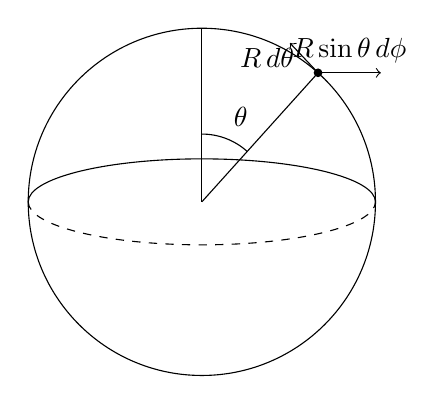
\begin{tikzpicture}[scale=1.05]
  \draw (0,0) circle (2.1);
  \draw[dashed] (-2.1,0) arc (180:360:2.1 and 0.52);
  \draw (2.1,0) arc (0:180:2.1 and 0.52);
  \coordinate (P) at (48:2.1);
  \fill (P) circle (1.5pt);
  \draw (0,0) -- (0,2.1);
  \draw (0,0) -- (P);
  \draw (0,0.82) arc (90:48:0.82);
  \node at (0.47,1.03) {\(\theta\)};
  \draw[->] (P) -- ++(-0.34,0.36)
    node[midway,left] {\(R\,d\theta\)};
  \draw[->] (P) -- ++(0.76,0)
    node[midway,above] {\(R\sin\theta\,d\phi\)};
\end{tikzpicture}
\caption{Reconstrucción clara de los segmentos diferenciales locales utilizados para obtener \eqref{eq:sphere-metric}.}
\end{figure}

Ningún cambio global de coordenadas convierte \eqref{eq:sphere-metric} en una matriz euclídea constante. Un observador bidimensional puede descubrirlo de manera intrínseca: un triángulo suficientemente grande formado por geodésicas tiene una suma de ángulos mayor que \(180^\circ\). Hemos llegado así al criterio útil. Los coeficientes variables no implican por sí solos que haya curvatura. La curvatura es el impedimento para encontrar coordenadas que hagan constante la métrica en toda la región considerada.

\section{Del espaciotiempo curvo a la cosmología}

La relatividad general permite que el propio espaciotiempo tenga esta curvatura intrínseca. Una métrica \(g_{\mu\nu}\) dependiente de la posición aún puede ser un artefacto de las coordenadas, como ocurre en coordenadas polares; pero en un espaciotiempo realmente curvo, ninguna transformación de coordenadas elimina globalmente la variación.

\begin{figure}[H]
\centering
\includegraphics[width=0.70\textwidth]{lecture_08_figure_09.png}
\caption{Transición de los ejemplos con coordenadas especiales al elemento de línea general del espaciotiempo \(ds^2=g_{\mu\nu}(x)dx^\mu dx^\nu\).}
\lectureframe{00:48:40}
\end{figure}

No intentaremos abordar toda la maquinaria de las ecuaciones de Einstein. En su lugar, nos limitaremos a geometrías adecuadas para la cosmología: se supone que el espacio es homogéneo a escalas suficientemente grandes, aunque su geometría puede cambiar con el tiempo. Homogéneo significa que ningún lugar se distingue de otro. No significa plano: todos los puntos de una esfera son equivalentes y, sin embargo, la esfera es curva. Tampoco significa que carezca de estructura a todas las escalas.

\begin{classroomqa}
\audiencequestion{¿Cómo puede ser homogéneo el universo si las galaxias forman cúmulos, láminas y filamentos?}
\lecturerresponse{La afirmación se refiere a escalas en las que se ha promediado la distribución. Las estrellas, las galaxias y los cúmulos son muy heterogéneos. Al comparar regiones de cientos de millones de años luz de diámetro, esas estructuras se promedian y tienden a una distribución uniforme. El principio cosmológico es una hipótesis empírica de trabajo, no una necesidad lógica; diferencias sistemáticas suficientemente grandes, incluidas las diferencias direccionales en el fondo cósmico, podrían refutarlo.}
\end{classroomqa}

El segundo supuesto de gran escala de esta clase es que el espacio es plano. En un instante cósmico fijo, los triángulos suficientemente grandes parecen euclídeos: sus ángulos suman \(180^\circ\). Esta afirmación se refiere a la geometría del espacio tridimensional, no todavía a la curvatura del espaciotiempo tetradimensional.

\begin{classroomqa}
\audiencequestion{¿Qué significa simultaneidad para puntos separados por distancias cosmológicas, dado que su luz nos llega en momentos distintos?}
\lecturerresponse{No podemos colocar reglas entre galaxias lejanas ni observarlas de manera instantánea. Recibimos señales más tarde y reconstruimos la geometría de los sucesos emisores dentro de un modelo del espacio-tiempo. El procedimiento es indirecto, pero también lo son muchas mediciones geométricas en astronomía. La planitud significa que los grandes triángulos reconstruidos no presentan excesos ni déficits angulares detectables en la escala estudiada.}
\end{classroomqa}

\section{Coordenadas comóviles y el factor de escala}

Imaginemos una cuadrícula cartesiana trazada sobre el flujo de galaxias a gran escala. Cada galaxia conserva su etiqueta de coordenadas mientras la cuadrícula se expande. Esa etiqueta no es una distancia en metros, sino una dirección. Un factor de conversión que depende del tiempo transforma las separaciones de coordenadas en separaciones físicas.

\begin{figure}[H]
\centering
\begin{tikzpicture}[>=Latex,scale=0.86]
  \foreach \x in {0,0.65,1.3,1.95,2.6} {
    \draw[gray!65] (\x,0) -- (\x,2.2);
  }
  \foreach \y in {0,0.55,1.1,1.65,2.2} {
    \draw[gray!65] (0,\y) -- (2.6,\y);
  }
  \fill[blue!65!black] (0.65,0.55) circle (2pt);
  \fill[red!70!black] (1.95,1.65) circle (2pt);
  \node[below] at (1.3,-0.2) {comoving labels at \(t_1\)};
  \draw[->,very thick] (3.0,1.1) -- (4.0,1.1)
    node[midway,above] {\(a(t)\) grows};
  \foreach \x in {4.4,5.5,6.6,7.7,8.8} {
    \draw[gray!65] (\x,0) -- (\x,2.2);
  }
  \foreach \y in {0,0.55,1.1,1.65,2.2} {
    \draw[gray!65] (4.4,\y) -- (8.8,\y);
  }
  \fill[blue!65!black] (5.5,0.55) circle (2pt);
  \fill[red!70!black] (7.7,1.65) circle (2pt);
  \node[below] at (6.6,-0.2) {same labels at \(t_2\)};
\end{tikzpicture}
\caption{Las direcciones comóviles permanecen fijas mientras crece la separación física de la cuadrícula de coordenadas.}
\end{figure}

La homogeneidad espacial exige el mismo factor de conversión en todas partes en un instante dado. La planitud espacial permite que la parte espacial de la métrica sea cartesiana. El elemento de línea resultante es
\begin{equation}
  d\tau^2
  =dt^2-a^2(t)\left(dx^2+dy^2+dz^2\right).
  \label{eq:flrw-flat}
\end{equation}
Esta es la métrica cosmológica homogénea espacialmente plana en coordenadas comóviles. Podemos elegir que \(x,y,z\) sea adimensional y asignar unidades de longitud a \(a(t)\). Otra convención puede incorporar las dimensiones en las coordenadas y hacer que \(a\) sea adimensional; solo importa el producto.

\begin{figure}[H]
\centering
\includegraphics[width=0.76\textwidth]{lecture_08_figure_10.png}
\caption{La métrica cosmológica espacialmente plana, tal como queda escrita en la pizarra, con el factor común \(a^2(t)\) multiplicando las tres direcciones espaciales.}
\lectureframe{01:03:15}
\end{figure}

Si \(a\) fuera constante, podríamos absorberlo reescalando \(x,y,z\), y \eqref{eq:flrw-flat} sería el espaciotiempo ordinario de Minkowski en otras unidades. Su dependencia temporal es el ingrediente no trivial.

\begin{classroomqa}
\audiencequestion{Si se expande la cuadrícula de coordenadas, ¿por qué no se expanden con ella las reglas, los átomos y las galaxias?}
\lecturerresponse{La métrica describe el flujo cósmico medio, no una fuerza que obligue a todos los sistemas ligados a seguirlo. Las fuerzas electromagnéticas mantienen unidas una regla y un átomo; la autogravedad mantiene unida una galaxia. En las escalas pequeñas, esos efectos de ligadura dominan sobre la expansión de fondo, extremadamente débil. Las galaxias cercanas también pueden apartarse del flujo de Hubble: Andrómeda es atraída hacia la Vía Láctea. Los estudios detallados de la ligadura galáctica muestran que la materia visible por sí sola es insuficiente, lo que constituye uno de los argumentos a favor de la materia oscura.}
\end{classroomqa}

\begin{classroomqa}
\audiencequestion{¿Por qué el factor de escala no es en sí una fuerza que empuje a las galaxias a separarse?}
\lecturerresponse{En la convención actual tiene dimensiones de longitud, no de fuerza. Pensemos en una bala de cañón lanzada hacia arriba. Una vez lanzada, su movimiento hacia afuera es inercial; la gravedad modifica ese movimiento al reducir su rapidez o hacerla regresar. Del mismo modo, la expansión es un estado de movimiento. La cuestión dinámica es cómo la gravedad y otras fuentes modifican \(\dot a\) y \(\ddot a\), no qué fuerza hace falta para mantener \(a\) en movimiento.}
\end{classroomqa}

La expectativa anterior era que la gravedad atractiva debía desacelerar la expansión. Para cuando se impartió esta clase, las pruebas astronómicas ya habían mostrado que, en cambio, la expansión reciente se acelera, lo que significa que la dinámica completa incluye algo más que materia ordinaria atractiva. Dejaremos ese asunto para más adelante, una vez establecida la estructura geométrica.

\section{La ley de Hubble}

Consideremos dos galaxias comóviles cuya separación fija en coordenadas es \(\Delta x\). En un mismo instante cósmico, su distancia física es
\begin{equation}
  D(t)=a(t)\,\Delta x.
  \label{eq:physical-distance}
\end{equation}
Derivemos respecto del tiempo manteniendo fijas las etiquetas comóviles:
\begin{align}
  V(t)
    &=\dot D(t)
      =\dot a(t)\,\Delta x \nonumber\\
    &=\frac{\dot a(t)}{a(t)}D(t).
  \label{eq:hubble-derivation}
\end{align}
Definamos
\begin{equation}
  H(t)=\frac{\dot a(t)}{a(t)}.
  \label{eq:hubble-parameter}
\end{equation}
Entonces
\begin{equation}
  V(t)=H(t)D(t).
  \label{eq:hubble-law}
\end{equation}
En un instante cósmico dado, el mismo \(H(t)\) se aplica en todas partes; de lo contrario, el espacio no sería homogéneo. La velocidad de recesión es proporcional a la distancia porque todos los intervalos de la cuadrícula comóvil se estiran a la misma tasa fraccional.

\begin{figure}[H]
\centering
\includegraphics[width=0.73\textwidth]{lecture_08_figure_11.png}
\caption{Distancia física \(D=a\Delta x\) y su derivada temporal, en la deducción de \(V=(\dot a/a)D\).}
\lectureframe{01:16:45}
\end{figure}

\begin{classroomqa}
\audiencequestion{Para una galaxia lejana, ¿hay que evaluar el parámetro de Hubble ahora o cuando se emitió la luz que observamos?}
\lecturerresponse{En la época que se describe. La luz de una galaxia lejana nos informa sobre un valor anterior de la expansión. Un análisis riguroso debe tener en cuenta la dependencia temporal de \(H\); usar en todas partes el valor actual es solo una aproximación local.}
\end{classroomqa}

\begin{classroomqa}¿Dónde están las unidades en \audiencequestion{\(D=a\Delta x\)?}
\lecturerresponse{Una opción práctica es tratar la etiqueta comóvil \(\Delta x\) como adimensional y dejar que \(a\) tenga unidades de longitud. También es posible llevar la cuenta de las unidades al revés. En cualquier caso, \(H=\dot a/a\) tiene dimensiones de inverso del tiempo.}
\end{classroomqa}

\section{La luz en coordenadas en expansión}

La luz sigue una trayectoria nula. A lo largo de ella, el intervalo de tiempo propio se anula:
\begin{equation}
  d\tau^2=0.
\end{equation}

\begin{classroomqa}
\audiencequestion{¿Por qué el intervalo es nulo para la luz?}
\lecturerresponse{Esa es la geometría que define un rayo de luz en la relatividad. Todo observador local en caída libre mide que la luz se mueve a \(c=1\), de modo que \(dt^2=d\ell^2\) localmente y el intervalo espaciotemporal se anula. Esto no significa que no transcurra tiempo coordenado para el observador que recibe la luz.}
\end{classroomqa}

Para un rayo que se mueve solo en la dirección \(x\),
\begin{equation}
  0=dt^2-a^2(t)\,dx^2.
\end{equation}
Si elegimos el rayo que se mueve hacia valores crecientes de \(x\),
\begin{equation}
  dt=a(t)\,dx,
  \qquad
  dx=\frac{dt}{a(t)},
  \qquad
  \frac{dx}{dt}=\frac{1}{a(t)}.
  \label{eq:null-ray}
\end{equation}

\begin{figure}[H]
\centering
\includegraphics[width=0.64\textwidth]{lecture_08_figure_12.png}
\caption{La condición nula en la métrica en expansión y la ecuación resultante para el rayo de luz comóvil \(dx=dt/a(t)\).}
\lectureframe{01:23:45}
\end{figure}

La velocidad de coordenadas \(dx/dt\) disminuye a medida que crece el factor de escala. Esto no significa que la luz se ralentice localmente. Una unidad de distancia en coordenadas comóviles representa una distancia física cada vez mayor, por lo que cambia el valor numérico de la velocidad de coordenadas, mientras que toda medición local sigue dando \(c=1\).

\section{Por qué importa la dependencia temporal}

Ahora resulta inevitable la cuestión geométrica central: ¿cómo varía \(a(t)\)? La analogía es la de un proyectil cuya posición se conoce en un instante. Para determinar su trayectoria futura hace falta una ecuación de movimiento. En cosmología, la dinámica gravitatoria proporcionará la ecuación para \(a(t)\).

\begin{classroomqa}
\audiencequestion{¿Por qué dar prioridad a la pregunta de si \(a(t)\) cambia, frente a la pregunta, igualmente legítima, de si, por ejemplo, la carga del electrón cambia con el tiempo?}
\lecturerresponse{No hay ninguna jerarquía lógica. Un cambio medido en la carga del electrón sería enormemente importante. Nos centramos en \(a(t)\) porque las observaciones ya nos indican que las separaciones cósmicas cambian, mientras que la carga del electrón parece constante. Geométricamente, una \(a\) constante podría eliminarse mediante un cambio de unidades espaciales y dejaría el espacio-tiempo plano; una \(a\) dependiente del tiempo no puede eliminarse de ese modo.}
\end{classroomqa}

Antes de medir la recesión de galaxias lejanas, hace falta este marco geométrico para precisar qué se mide. En la aproximación más burda, una fuente de luminosidad conocida parece más tenue cuanto más lejos está, porque su luz se distribuye sobre un área mayor; por otra parte, el desplazamiento de líneas espectrales atómicas conocidas da un corrimiento al rojo y, por tanto, un indicador de recesión. Hubble combinó estimaciones de distancia con corrimientos al rojo para descubrir la proporcionalidad \eqref{eq:hubble-law}, aunque el valor numérico inicial del coeficiente era considerablemente erróneo. Las escaleras de distancias modernas y los cálculos relativistas de propagación de la luz son mucho más elaborados, pero la pareja conceptual sigue siendo la misma: distancia y corrimiento al rojo.

\section{El tiempo de Hubble y la estimación de la edad}

La ley de Hubble encierra una estimación sencilla. Fijemos la velocidad de recesión actual de una galaxia y extrapolemos uniformemente el movimiento hacia atrás en el tiempo. El tiempo necesario para recorrer la distancia actual sería
\begin{equation}
  t=\frac{D}{V}.
\end{equation}
Usando \(V=HD\),
\begin{equation}
  t=\frac{D}{HD}=\frac{1}{H}.
  \label{eq:hubble-time}
\end{equation}
La distancia se cancela, así que cualquier par de galaxias comóviles da el mismo tiempo aproximado. Susskind detecta y corrige aquí un fácil error verbal. El supuesto no es que \(H\) permanezca constante. Se trata de extrapolar hacia atrás una velocidad de recesión particular como si permaneciera constante.

\begin{figure}[H]
\centering
\includegraphics[width=0.66\textwidth]{lecture_08_figure_13.png}
\caption{La estimación del tiempo de Hubble \(H^{-1}=D/(HD)=D/V\), en la que la distancia se cancela en la extrapolación hacia atrás.}
\lectureframe{01:33:45}
\end{figure}

Por tanto, el inverso del parámetro de Hubble es una escala de tiempo, pero no es automáticamente la edad exacta del universo. En un modelo en el que la expansión se desacelera y domina la materia, invirtamos la velocidad actual y dejemos que la gravedad atraiga las galaxias. Se encuentran antes de lo que lo harían a velocidad uniforme, así que el valor actual de \(H^{-1}\) sobreestima la edad. La clase da una edad refinada de aproximadamente \(13.5\) mil millones de años, cercana al tiempo de Hubble, pero no idéntica a él.

\begin{classroomqa}
\audiencequestion{Si no hay expansión de Hubble dentro de nuestra galaxia, ¿qué significa hacer retroceder todas las galaxias hasta que colapsen?}
\lecturerresponse{La descripción homogénea deja, con el tiempo, de representar la historia real de las estructuras ligadas. Al avanzar el tiempo, las pequeñas fluctuaciones crecen gravitatoriamente y forman galaxias y cúmulos. Para invertir literalmente la película habría que invertir cada movimiento microscópico y reducir la entropía; invertir simplemente el flujo medio de Hubble no deshace la formación de estructuras. La extrapolación hacia el pasado es una estimación cosmológica aproximada, no una película en la que cada estrella recorra de nuevo su trayectoria.}
\end{classroomqa}

\begin{classroomqa}
\audiencequestion{¿Puede un experimento distinguir entre una distancia intergaláctica que aumenta y una regla que se encoge?}
\lecturerresponse{Solo son observables las razones adimensionales. Lo que se mide es que aumenta la distancia entre galaxias dividida por una longitud atómica o un patrón de laboratorio. Por convención, mantenemos fijos los parámetros de la física atómica y molecular y decimos que el universo se expande. También se podría elegir la separación intergaláctica como patrón y describir los átomos, los protones y las reglas como objetos que se encogen. La física de la razón no cambiaría.}
\end{classroomqa}

Esa convención es natural porque las reglas están hechas de átomos y su tamaño está determinado por parámetros que parecen constantes. En última instancia, un metro equivale a un gran número de longitudes microscópicas. Si mantenemos fijos esos patrones microscópicos, obtenemos la afirmación habitual de que \(a(t)\) crece.

\begin{classroomqa}
\audiencequestion{¿Es \eqref{eq:flrw-flat} la única métrica compatible con la homogeneidad y la planitud espaciales?}
\lecturerresponse{Solo salvo transformaciones de coordenadas. La afirmación precisa es que, bajo esos supuestos y con una elección adecuada del tiempo cósmico y de las coordenadas espaciales comóviles, se puede llevar la métrica a esta forma. Otro sistema de coordenadas puede hacer que el mismo espacio-tiempo parezca muy distinto.}
\end{classroomqa}

\begin{classroomqa}
\audiencequestion{Cuando la separación extrapolada hacia el pasado llega a cero, la ley de Hubble también da velocidad nula. ¿Eso impide que las galaxias lleguen a encontrarse?}
\lecturerresponse{No. El valor de \(H\) inferido hoy no se mantiene fijo durante toda la extrapolación hacia el pasado. En las soluciones expansivas habituales, \(H(t)\) era mucho mayor en épocas anteriores. La estimación \(H_0^{-1}\) se obtiene prolongando uniformemente la velocidad actual solo para calcular una escala; los valores reales de \(a(t)\) y \(H(t)\), así como las velocidades, deben determinarse a partir de la dinámica.}
\end{classroomqa}

\section{El teorema de las capas de Newton y la dinámica cosmológica}

Para descubrir la dinámica, distribuyamos las galaxias como un medio homogéneo. Elijamos una galaxia como origen y otra con etiqueta comóvil \(x\). Esta elección no confiere ningún privilegio físico; la homogeneidad exige que la ecuación final sea la misma alrededor de cualquier galaxia. El radio físico de la segunda galaxia es
\begin{equation}
  R(t)=a(t)x.
  \label{eq:radius-ax}
\end{equation}

A primera vista, para hallar su aceleración gravitatoria parece necesario sumar la atracción de todas las galaxias de un universo enorme. El teorema de las capas de Newton simplifica el problema:

\begin{proposition}[Newton's shell theorem]Para una fuerza inversamente proporcional al cuadrado de la distancia y una distribución de masa con simetría esférica, la materia situada fuera de una esfera que pasa por el punto de prueba no ejerce ninguna fuerza neta. La materia dentro de la esfera actúa sobre el punto de prueba como si toda la masa encerrada estuviera concentrada en el centro.
\end{proposition}

\begin{figure}[H]
\centering
\includegraphics[width=0.70\textwidth]{lecture_08_figure_14.png}
\caption{La distribución homogénea de galaxias, una galaxia de prueba con etiqueta comóvil \(x\) y la esfera cuya masa encerrada es la única que determina su movimiento radial.}
\lectureframe{01:50:05}
\end{figure}

\begin{figure}[H]
\centering
\begin{tikzpicture}[scale=0.94,>=Latex]
  \draw[gray!65] (0,0) circle (2.35);
  \foreach \p in {
    (-1.5,0.8),(-1.2,-0.8),(-0.8,1.5),(-0.6,0.35),(-0.3,-1.45),
    (0.15,1.05),(0.35,-0.55),(0.7,1.65),(0.9,0.45),(1.25,-0.9),
    (1.65,0.95),(-1.75,-0.2),(1.8,-0.15)} {
    \fill[black!55] \p circle (1.15pt);
  }
  \fill[blue!65!black] (0,0) circle (2pt)
    node[below left] {chosen origin};
  \fill[red!70!black] (2.35,0) circle (2.2pt)
    node[right] {test galaxy};
  \draw[->,thick] (0,0) -- (2.32,0)
    node[midway,above] {\(R=a(t)x\)};
  \draw[<->] (-2.35,-2.55) -- (2.35,-2.55)
    node[midway,below=4pt] {only the enclosed mass contributes};
\end{tikzpicture}
\caption{Reconstrucción clara del esquema del teorema de las capas. El origen se elige por comodidad; no es el centro del universo.}
\end{figure}

El problema cosmológico de muchos cuerpos se ha convertido así en el conocido problema de un cuerpo: un proyectil que se mueve radialmente bajo la atracción de la masa encerrada en la esfera que lo contiene. La ecuación de Newton determinará cómo se acelera \(R=a x\) y, por tanto, \(a(t)\). La clase se detiene deliberadamente antes de realizar ese cálculo. En la próxima sesión se deducirá la cosmología más sencilla dominada por la materia, en vez de introducir su resultado a escondidas en el planteamiento geométrico.

\section{Preguntas finales: la luz, el Big Bang y la curvatura}

La clase formal ha terminado, pero las preguntas finales ponen de manifiesto varias imágenes engañosas y forman parte de la física, no son un apéndice.

\begin{classroomqa}
\audiencequestion{Si la luz de objetos muy distantes se emitió cuando el universo era mucho más pequeño, ¿por qué ahora parece venir de tan lejos? Y si el universo primitivo era compacto, ¿por qué no es observable en su totalidad?}
\lecturerresponse{Hay que resolver la ecuación de los rayos nulos en coordenadas en expansión. Cuando \(a(t)\) es muy pequeño, \(dx/dt=1/a(t)\) es muy grande: la luz atraviesa un gran intervalo comóvil mientras localmente sigue moviéndose a \(c=1\). A medida que \(a(t)\) crece, disminuye su velocidad coordenada comóvil. El punto preciso de emisión y el tamaño de la región observable dependen de toda la historia de \(a(t)\), así que se pospone una respuesta numérica hasta haber resuelto una cosmología concreta.}
\end{classroomqa}

\begin{figure}[H]
\centering
\includegraphics[width=0.72\textwidth]{lecture_08_figure_15.png}
\caption{Un rayo de luz en el plano \((x,t)\): casi horizontal en coordenadas comóviles cuando \(a(t)\) es pequeño, y luego cada vez más inclinado a medida que crece el factor de escala.}
\lectureframe{01:56:20}
\end{figure}

Al integrar \eqref{eq:null-ray} queda explícito el cálculo que se había pospuesto:
\begin{equation}
  \Delta x
  =\int_{t_{\mathrm e}}^{t_0}\frac{dt}{a(t)}.
  \label{eq:comoving-light-distance}
\end{equation}
Que la integral alcance distancias comóviles arbitrariamente grandes cuando \(t_{\mathrm e}\) se aproxima al comienzo depende de la forma que tenga \(a(t)\) en los primeros tiempos.\editorialnote{La ecuación \eqref{eq:comoving-light-distance} es la forma integrada de la ecuación de la pizarra \(dx=dt/a(t)\). Hace explícito el cálculo que la clase deja para la próxima sesión, sin elegir un factor de escala particular.}

\begin{figure}[H]
\centering
\begin{tikzpicture}[scale=0.92,>=Latex]
  \draw[->] (0,0) -- (6.4,0) node[right] {\(x\)};
  \draw[->] (0,0) -- (0,4.6) node[above] {\(t\)};
  \draw[thick,blue!65!black]
    plot[smooth] coordinates {(0,0.18) (1.65,0.42) (2.65,1.05)
      (3.35,2.05) (3.85,3.25) (4.05,4.25)};
  \fill[red!70!black] (4.05,4.25) circle (2pt)
    node[right] {reception today};
  \draw[dashed] (4.05,0) -- (4.05,4.25);
  \node[align=left] at (1.65,3.25)
    {\(\displaystyle \frac{dx}{dt}=\frac1{a(t)}\)\\
     large when \(a\) is small};
\end{tikzpicture}
\caption{Versión limpia de la construcción del rayo de luz en coordenadas comóviles. La pendiente cambiante es un efecto de las coordenadas, no un cambio en la velocidad local de la luz.}
\end{figure}

\begin{classroomqa}
\audiencequestion{¿El Big Bang expulsó materia desde un punto, de modo que ahora debería encontrarse en una capa o un anillo en expansión?}
\lecturerresponse{No. El modelo comienza con un espacio homogéneo y extremadamente denso. Todas las separaciones a gran escala aumentan; la materia no sale disparada a través de un espacio vacío preexistente desde un centro privilegiado. Un globo cubierto uniformemente de puntos ofrece una analogía bidimensional útil: al expandirse, aumentan las separaciones entre todos los puntos, mientras la superficie sigue poblada uniformemente. Incluso es posible que el espacio sea infinito en todo instante positivo; la expansión no implica que empezara como una bola finita dentro de otra cosa.}
\end{classroomqa}

\begin{classroomqa}
\audiencequestion{¿La gravedad misma era más débil o más fuerte durante la expansión?}
\lecturerresponse{En esta discusión, la constante de Newton \(G\) se mantiene fija. Sin embargo, la fuerza cambia porque cambian las separaciones y las densidades encerradas. En épocas anteriores, la misma galaxia comóvil estaba físicamente más cerca y la materia homogénea era más densa, así que la desaceleración gravitatoria era mayor. Esto es precisamente lo que se pretende cuantificar con el cálculo basado en el teorema de las capas esféricas.}
\end{classroomqa}

Por último, no hay que confundir la curvatura espacial con la expansión. Una pequeña región de la Tierra parece plana porque su tamaño es diminuto comparado con el radio terrestre. Midiendo triángulos suficientemente grandes, se puede detectar un exceso angular o establecer un límite inferior para el radio de curvatura. La astronomía realiza un experimento análogo con triángulos enormes. Según el lenguaje observacional empleado en la clase de 2006, no se detectó curvatura en toda la región visible, por lo que cualquier radio de curvatura tenía que ser considerablemente mayor que esa región. Esto no demuestra que el universo sea exactamente plano; establece un límite para cuán curvada puede ser la parte accesible.

Para una esfera, la curvatura intrínseca varía como \(R^{-2}\). Por tanto, una esfera que crece se vuelve localmente más plana. Del mismo modo, si un universo homogéneo tiene curvatura espacial distinta de cero, la expansión aumenta su radio de curvatura y reduce la curvatura visible en cualquier región local de tamaño fijo.
\editorialnote{La dependencia \(R^{-2}\) es la forma cuantitativa estándar de expresar lo que dice la clase: la curvatura numérica disminuye a medida que crece una esfera.}

\begin{classroomqa}
\audiencequestion{Si el espacio está curvado, ¿tiene que contraerse una componente del universo mientras otra se expande?}
\lecturerresponse{No. La curvatura espacial positiva, nula o negativa describe la geometría de cada sección de tiempo cósmico. La expansión o la contracción están determinadas por la evolución de \(a(t)\). Un universo curvado puede expandirse; uno plano puede contraerse. La expansión puede invertirse más adelante, igual que un proyectil que sube puede volver a caer, pero la curvatura no oculta una contracción simultánea. La cuestión dinámica es si el movimiento hacia afuera escapa a la atracción de la masa encerrada, vuelve a caer o se encuentra en el umbral crítico.}
\end{classroomqa}

Esa comparación con la velocidad de escape es la última idea de la clase desarrollada en la pizarra. La geometría ha proporcionado la métrica, la ley de Hubble y la ecuación del rayo de luz. El teorema de Newton ha reducido la dinámica a la masa dentro de una esfera. La próxima clase empieza exactamente donde esta debe terminar: con la ecuación que determina \(a(t)\) y con la pregunta de si la expansión escapa, vuelve a contraerse o permanece en el límite crítico.
